\chapter{Hierarchical pruning based automatic neuron tracing methods} \label{chpt:auto-nt}
In this chapter we focus on neuron tracing for 3D light-microscopic images (often confocal or multi-photon laser scanning microscopic images). Taking a 3D gray-scale image as the input, a neuron tracing method produces the digital representation of the morphology of the neuron(s) in this image.

\section{Background}
\subsection{Diadem challenge}
The shape of neuron is much related to neuronal function. Due to the lack of efficient tools and method, the shape of neurons are mostly obtained manually. To raise awareness of the problem of automated neuronal reconstruction, a competition for neuron reconstruction is set up by the Allen institue for Brain Science and the Janelia Farm Research Campus of the Howard Huges Medical Institute (HHMI). It is called Diadem Challenge.
\subsection{APP1 method}
\section{APP2 method}
\subsection{Overview of APP2}
In many previous studies, the 3D reconstructed morphology of a neuron is described using a tree graph $G$.  $G$ has a root node that corresponds to the seed location for reconstruction, which in many cases also corresponds to the soma of a neuron. $G$ may also contain many leaf nodes, branching nodes and other internodes.

An important idea in the recent all-path-pruning (APP) method \cite{peng2011automatic} is to first generate an over-reconstruction from the image to capture all possible signal/pixels of a neuron, and then uses an optimal pruning procedure to remove the majority of spurs in this over-reconstruction to produce a final succinct representation of the neuron, with a maximum coverage of all neuron signal. The pruning process starts from leaf nodes of the over-reconstruction. A "coverage" test is iteratively conducted to check whether or not any of them have been "covered" (i.e. has significant signal overlap) by other nodes. The nodes that are covered by others will be removed; otherwise they will be kept. A similar process is also applied to all internodes. The entire procedure is repeated until a most succinct representation that maximizes the signal coverage has been produced. While the termini-first-search approach in APP is effective, it needs multiple iterations, which could still be time-consuming even the algorithm itself has linear-time complexity to the number of reconstruction nodes. In addition, APP does not consider how to best preprocess an input image to optimize the tracing result. 

APP2 follows the basic framework of APP. However, it enhances the key components of the original method. In short, APP2 consists of three steps in Fig.\ref{fig:autont-fig1}b, c, and d: (1) gray-weighted distance transform (Section \ref{sec:gwdt}); (2) construction of an initial, over-reconstruction of the traced neuron (Section \ref{sec:init-nt}); and (3) pruning of the over-reconstruction in hierarchical order (Section \ref{sec:nt-hp}). The detail of APP2 is described as follows.

\begin{figure}[htbp]
\centering
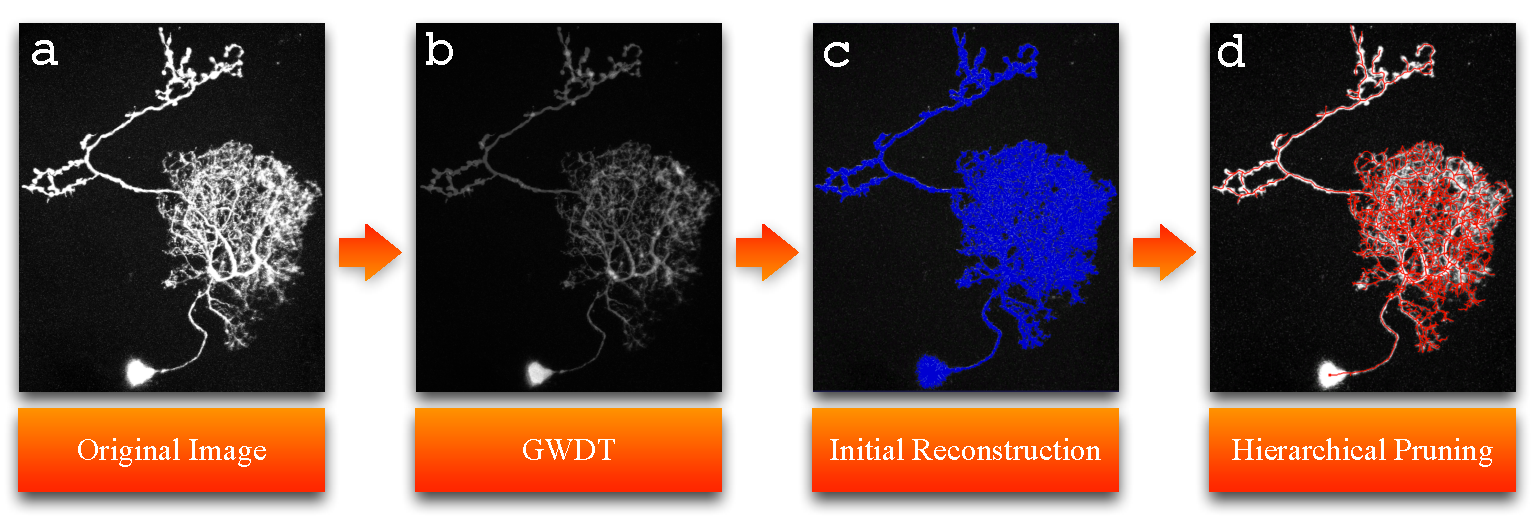
\includegraphics[width=1.0\textwidth]{images/autont_fig1}
\caption[Schematic illustration of APP2 neuron tracing method]{Schematic illustration of APP2 neuron tracing method. GWDT: gray-weighted distance transform. In c and d, the reconstructions are color-rendered and overlaid on top of the image data for better visualization. Raw image: Courtesy of Chiang lab.}
\label{fig:autont-fig1}
\end{figure}
\subsection{GWDT: Gray-Weighted Distance transfrom} \label{sec:gwdt}
To enhance the quality of an initial neuron reconstruction, in APP2 we apply the distance transform (DT) to the input image. In case of an image region that have relatively "flat" intensity, DT is able to create a gradient of image intensity: close to the center of this region the image intensity is large, and close to the boundary the intensity is small. We call this ICDB principle, which stands for "\emph{i}ncrease the intensity in the \emph{c}enter and \emph{d}ecrease the intensity near \emph{b}oundary". It would help to build a high quality initial reconstruction by forcing the shortest path to go through the skeleton of the neuron.

However, the conventional distance transform is only applicable to a binary image that is produced by thresholding a gray-scale image. An unsuitable threshold may under or over segment the image. Here we propose a gray-weighted distance transform method for gray-scale image (GWDT) directly. In the conventional distance transform, the distance value for each image pixel is defined as the minimal Euclidean distance to background pixels. In GWSDT, the distance value for each pixel is defined as the sum of image pixels’ intensity along the shortest path to background. This is intrinsically similar to the gray weighted distance transform that has been previously defined by Rutovitz (1968)\cite{rutovitz1968data} and its variants. Most of the previous work and implementations (such as the recently released Matlab toolbox function) were limited to 2D cases, while our method and implementation are general for N-dimensional data ($N = 2,3,\ldots$). In the following we describe our fast implementation within FM framework.   

The distance value defined in GWSDT fits the ICDB principle. To use GWSDT, we often use a very low threshold value (e.g. the average intensity of an entire image). Any image pixels that have intensity value no greater than this threshold are called "background pixels". We first set all image background pixels as "seeds", then compute the distances from these seed pixels to other pixels. This process is similar to region growing, and thus is formulated within the FM framework in Chapter \ref{chpt:fm}. Here, the edge distance between consecutive image pixel vertices is defined as,
\begin{equation}
e(x,y)=|(|x-y|)|.I(y)
\end{equation}
Where $x$ is source vertex, $y$ is target vertex, $I(y)$ is the intensity of image pixel $y$. Let $d(x)$ denote the distance value of $x$. In the initialize step, we set
\begin{equation}
d(x)= \left\{
\begin{array}{rl}
I(x)  & x \in {background} \\
\infty &    x \notin {background } 
\end{array}
\right.
\end{equation}
We will set all background pixels as seeds. The neighbor pixels of all seeds will be set as the initial \emph{TRIAL} vertices and are pushed into the priority queue. In the growing step we will apply the formula,
\begin{equation}
d(x)=\min⁡{d(y)+ I(x)},y \in \{\mbox{neighbors of }x\}
\end{equation}
to refresh the distance value from background to skeleton center.

\textbf{Automated Soma detection}: We find that GWSDT method provides a way to detect the soma position of a neuron. Normally the soma has the maximum distance-transformed value (e.g. see results in \ref{}).

\subsection{Initial neuron reconstruction}\label{sec:init-nt}
In APP, the initial neuron reconstruction is essentially produced via finding the single-source (often from the soma) shortest path to all remaining foreground image pixels. APP uses Dijkstra’s algorithm, which needs to first build a graph of all foreground pixels and then find the shortest path from each pixel to the seed. For very large 3D image stacks, this approach may need a large amount of computer memory to hold the graph. In APP2, we present a new method to use FM to construct the initial reconstruction (Fig. \ref{fig:autont-fig2}), without the need to create such a large graph. 

In our implementation, we add a parental map par on the FM as described in Chapter \ref{chpt:fm} to generate the shortest path tree from a single source s.  Initially, the parent of each image pixel $x$ is set to be itself, i.e. $par(x)=x$. Then, for each neighbor pixel $y$ of $s$, we set them to have label "\emph{TRIAL}", and at the same time $par(y)=s$. In the recursive step, for the minimum pixel $x$ and each of its neighbor $y$, we set
\begin{equation}
par(y) = \left\{
\begin{array}{cl}
x & \mbox{if }y\mbox{ is }FAR \\
x & \mbox{if }d(x)+ e(x,y)< d(y)
\end{array}
\right.
\end{equation}

The edge distance e(x,y) is defined as the geodesic distance,
\begin{equation}
e(x,y)=\parallel x-y\parallel\cdot((g_I (x)+ g_I (y))/2)
\end{equation}
where the first item is Euclidean distance of the two pixels, and $g_I (.)$ in the second item is defined in the same form of APP \cite{peng2011automatic}, where $λ_I$ is a coefficient (set as 10 throughout our tests). 
\begin{equation}
g_I (x)=exp⁡(\lambda_I (1-I(x)/I_{max} )^2 )
\end{equation}
When FM has finished, we can build the initial reconstruction from the parental map.

In addition to the small working space needed, another useful property of FM for generating the initial reconstruction is that it can be stopped easily as needed. We consider two methods in APP2. First, the recursive step will stop when any background pixel becomes \emph{ALIVE}. This method prevents the marching process growing to any irrelevant area. Second, a user can optionally choose to specify some locations in advance (e.g. some special termini of a neuron) as additional priors; when all of these special locations have been labeled as \emph{ALIVE}, FM stops. The second method forces FM to reach these specified locations. Both methods are used in practice to generate complete initial reconstructions that cover signals as much as possible and thus make it easier to trace broken pieces or gaps in images. 

\begin{figure}[htbp]
\centering
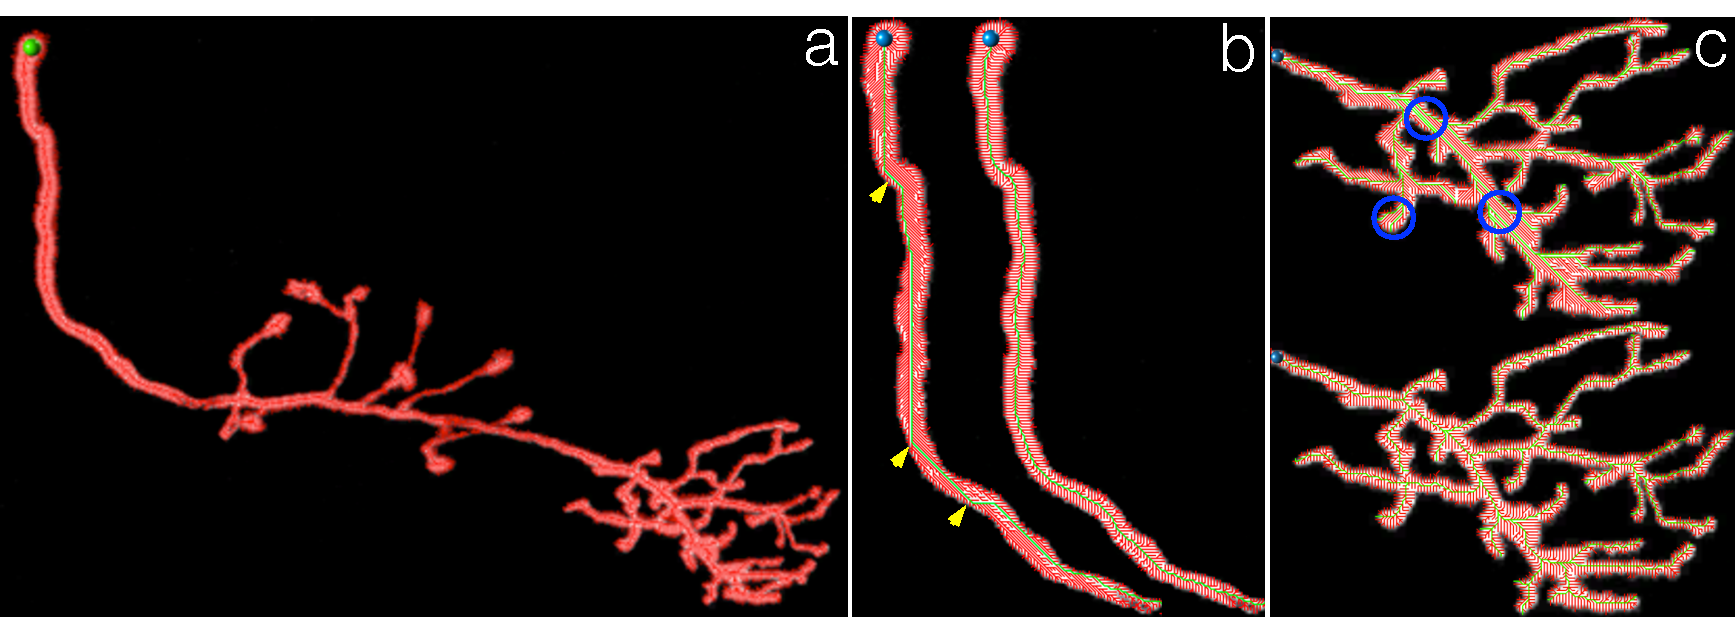
\includegraphics[width=1.0\textwidth]{images/autont_fig2}
\caption[Initial reconstruction based on GWDT and comparison results with or without GWDT]{Initial reconstruction based on GWDT (image: DIADEM OP1) and comparison results with or without GWDT. (a) The main GWDT-based skeleton (the major mid-curves) of the tracing implies a good tracing.  Sphere: the seed location. (b) left: out-of-center problem without GWDT preprocessing; right:  main structure goes to the neuron center with GWDT preprocessing . (c) top: parallel-path problem without GWDT preprocessing; bottom: parallel paths disappear after GWDT preprocessing.}
\label{fig:autont-fig2}
\end{figure}
\subsection{Hierarchical pruning}\label{sec:nt-hp}
Fig. \ref{fig:autont-fig2}a displays an example of an initial reconstruction of neuron. It is essentially a tree graph with a number of spurs. The next step is to find the main skeleton of the tree by removing the unnecessary or redundant spurs. Here we propose a hierarchical pruning method that contains two steps: a hierarchical segments construction step and a recursive pruning step. 
\subsubsection{Hierarchical segments construction}
For simplicity, we call the initial reconstruction a "tree" in this section. We define a segment in the tree as a path connecting two branching nodes in the tree. In the hierarchical segments construction step, we order all segments in the tree from most important to the least important and thus generate a hierarchy of them. The “importance” of a segment is defined based on its length. The longer a segment, the more important it is. Obviously, there is no overlap between any pair of segments. To get the importance scores, we first find the longest path from the most distal leaf node to the source node (seed). We then delete this segment from the tree and find the second longest segment from the remaining parts in the original tree. We iterate this process until all segments have been sorted. 

We further improve the efficiency of the algorithm as follows. We observe that in our decomposition of a tree, each hierarchical segment starts from a leaf node. In addition, there is a one-to-one mapping relationship between each hierarchical segment to a leaf node. Therefore, in a refined algorithm, we construct the hierarchical segments in a bottom up order. First, we detect the segment from each leaf node to its nearest branch node (excluding the branch node). Each branch node connects to at least two such segments. Then we merge the branch node to the longest segment (called "joint-segment"). Next, the other segments originally connects to the branch node are set as child segments to the joint segment. We iterate this joint segment merging process until the seed node is reached. 
\subsubsection{Recursive pruning}
In the pruning step, from the pool of undeleted hierarchical segments we choose one segment at a time following the importance-score in decreasing order. Then, we extend the signal-coverage idea in APP to coverage ratio of this segment (see below). If the coverage ratio is larger than a threshold value (normally 75\%), we delete this segment and all its child-segments. Otherwise, we keep this chosen segment and mask the coverage area of the segment. We iterate this process until no segment can be removed.

The coverage area of a segment is defined as the merged coverage area of all nodes in the segment. The coverage area of a node is defined as the sphere area centered at the node, with an estimated radius of the node, which is computed using the method described in Peng et al \cite{peng2010v3d,peng2010automatic}.

The coverage ratio of a segment is defined as the ratio of the number of all masked nodes with respect to the total number of nodes in the segment. Further, we consider image pixels with different intensities should have different weights. Thus in our scheme, we use the image-pixel-intensity weighted coverage ratio, which is defined as the sum of intensity of all masked nodes divided by that of all nodes in the segment.
\section{Experimental results}
\subsection{Results between GWDT and Non-GWDT}
We compared the new GWDT step in APP2 to those generated without GWDT (see Fig. \ref{fig:autont-fig2}). It is clear that when GWDT is not used (left of Fig. \ref{fig:autont-fig2}b), the detected skeleton of the neuron is often skewed to one side of the shape. This is effectively avoided when GWDT is used (right of Fig. \ref{fig:autont-fig2}b); the respective skeleton best covers the neurite signal in a balanced way.

Fig. \ref{fig:autont-fig2}c shows that for complex branching patterns, the shortest path algorithm could easily produce "parallel paths" when GWDT is not used (top of Fig. \ref{fig:autont-fig2}c). This problem is also clearly overcome after GWDT is applied to the image (Fig. \ref{fig:autont-fig2}c bottom). For this test image, the overall morphology of the GWDT-based result (Fig. \ref{fig:autont-fig2}c bottom) appears to be more reasonable than the non-GWDT result.

Of course, when GWDT is not invoked, APP2 can run faster (Table \ref{tab:autont-tab1}), although the accuracy might be compromised in a way similar to Fig. \ref{fig:autont-fig2}.

\begin{table} \label{tab:autont-tab1}
  \caption{The numbers of tree-segments pruned by APP2 and APP when sequentially applying APP2 or APP methods in pruning}
\begin{center}
 \begin{tabular}{ccccc}
    \hline
	\multirow{2}{*}{Neuron image} &\multicolumn{2}{c}{First APP2 then APP} & \multicolumn{2}{c}{First APP then APP2}\\ \cline{2-5}
	 &APP2 & APP & APP & APP2\\ \hline
	OP1 fly & 9421& 0 & 9180& 246 \\ \hline
Chiang fly	& 42069	& 3 &	34185 &	6529\\ \hline
Dragonfly C147 &	411	& 0	& 252 &	159\\ \hline
Dragonfly C150 &	10082 &	1 &	6709 &	3410\\ \hline
Dragonfly C152 &	662	& 0 & 	588 &	74\\ \hline
Dragonfly C154 &	969	& 0	& 598	& 368\\ \hline
Dragonfly C157 &	6084 &	3	& 2350 &	3731\\ \hline
Dragonfly C158 &	60331 &	25 &	44216 &	16499\\ \hline
Dragonfly C159 &	395	& 0	& 266 &	129\\ \hline
Dragonfly C160 &	7787 &	0	& 2639 &	5118\\ \hline
Dragonfly C161 &	45409 &	22 &	31098 &	14606\\ \hline
Dragonfly C162 &	328	& 1	& 293 &	38\\ \hline
Dragonfly C165 &	2854 &	1 & 	744 &	2108\\ \hline
Dragonfly C168 &	2537 &	0 &	1777 &	753\\ \hline
Dragonfly C169 &	981	& 0	& 720 &	253\\ \hline
Dragonfly C171 &	2260 &	0 &	1509 &	750\\ \hline
Dragonfly C173 &	2189 &	0 &	1662 &	518\\ \hline
Dragonfly C175 &	4830 &	0 &	3239 &	1555\\ \hline
Dragonfly C179 &	1905 &	0 &	1378 &	518\\ \hline
Dragonfly C180 &	456	& 0	& 350 &	106\\ \hline
Dragonfly C183 &	195	& 0	& 145 &	50\\ \hline
Dragonfly C188 &	2785 &	0 &	2401 &	381\\ \hline
Dragonfly C189 &	383	& 0	& 331 &	55\\ \hline
Dragonfly C190 &	39	& 0	& 25 &	14\\ \hline
Dragonfly C192 &	1048 &	0 &	832 &	215\\ \hline
Dragonfly C193 &	624	& 0	& 464 &	163\\ \hline
Dragonfly C194 &	1243 &	0 &	815 &	426\\ \hline
    \end{tabular}
\end{center}
\end{table}

\begin{table} \label{tab:autont-tab2}
\caption{Comparison of running time (seconds) of APP2 and APP on a few images. Testing is based on a MacPro laptop with 2.6GHz Intel Core i5}
\begin{center}
\begin{tabular}{cccc}
\hline
Image	& APP &	APP2 (w/ GWDT)	& APP2 (w/o GWDT) \\ \hline
Chiang fly & 149.7 &	28.9 &	12.6 \\ \hline
Dragonfly C154 &	31.6 &	6.9 &	1.6 \\ \hline
Dragonfly C168 &	48.8 &	7.9	& 1.9 \\ \hline
Dragonfly C171 &	44.2 &	10.2 &	2 \\ \hline
Dragonfly C190 &	32.6 &	7.6	& 1.3 \\ \hline
\end{tabular}
\end{center}
\end{table}

\subsection{Comparison with other methods}
We examined the robustness of APP2 by tracing images where signal were deleted \cite{peng2010automatic}. Three levels of signal deletion, 30\%, 60\% and 90\% were tested (Fig. \ref{fig:autont-fig3} and Fig. \ref{fig:autont-fig3-2}). We compared APP2 to several previous automated methods in the public domain, including APP \cite{peng2011automatic}, NeuronStudio \cite{rodriguez2008automated}, and SimpleTracing \cite{yang2013distance} , as well as the "ground truth" reconstruction, which was obtained by combining semi-automatic tracing and manual editing. To make a fair comparison, the reported results of competing methods correspond to the best possible parameters finetuned in our testing. 

We calculated several difference scores of the reconstructions produced by the automated methods and the "ground truth". These difference scores measure the "spatial distance" between a particular reconstruction and the ground truth, as well as the percentage of reconstruction elements that have significant, i.e. visible, distance to the nearest reconstruction elements in the "ground truth". These scores, as previously defined in Peng et al.\cite{peng2010v3d}, are called entire structure average (ESA), different structure average (DSA) and percent of different structure (PDS) for simplicity in this paper. 

Fig. \ref{fig:autont-fig3} shows that APP2 is able to achieve the lowest difference-scores among all methods. It actually consistently produced subpixel precision compared to other methods, such as NeuronStudio. For the DSA score, APP2 and APP are close to each other, but APP2 is better than APP in the ESA and PDS scores. 

\subsection{Improvement on APP}
Fig. \ref{fig:autont-fig3} indicates that the performance of APP2 is better, but still close to that of APP. While this observation is anticipated, it raises a natural question that how much APP2 will improve APP. In our design, the biggest difference between these two methods is how they prune the initial over-reconstructions. Therefore, we studied the ability of APP2 in pruning the initial reconstruction. We also compared the running speed of both methods.

We considered using either APP or APP2 to prune an initial re-construction, followed by using the other method (APP2 or APP) to check if there is any further redundancy in the reconstruction that can be removed. After applying this test to a number of complicated dragon fly neurons, we found that (Table \ref{tab:autont-tab1}) on average APP2 is able to prune most redundant segments in an initial reconstruction tree, leaving a very small portion of redundancy that can be detected by APP. On the other hand, when we apply APP first, APP2 is still able to remove many tree-segments. This shows the advantage of hierarchical pruning. In this sense, APP2 provides a complementary pruning scheme to the APP method.  

Table \ref{tab:autont-tab2} summarizes the running speed of APP2 versus APP for several testing images. It can be seen that APP2 is much faster on these images.

\subsection{Real applications in tracing different neuron images of different animals and from different labs}
We tested APP2 on a variety of real neuron data sets, including for instance the fruitfly neurons data used in DIADEM competition, the flycircuit.org database, and Janelia fly imagery database, as well as some very challenging dragonfly neuron data sets \cite{gonzalez2013eight} that have heavy noise. 
Fig. \ref{fig:autont-fig4} shows a few examples of tracing various data sets:
\begin{itemize}
\item[(a)]	For images that have very uneven image pixel intensity (e.g. Fig. 4c), APP2 is able to produce a complete reconstruction. 
\item[(b)]	For images that have fine branches (e.g. Fig. 4d), which are very easy to get missed by other tracing methods, APP2 is able to detect them reasonably well. 
\item[(c)]	For a neuron that may contain a big cell body (e.g. Fig. 4b), APP2 is able to detect the cell body automatically, and therefore reconstruct the entire morphology fully automatically.
\end{itemize}

\subsection{Large-scale reconstruction of single fruitfly neurons}
We applied APP2 to 678 3D 40x confocal images contributed by Chiang lab. Each image contains a single neuron labeled in a Drosophila brain. We ran both automatic soma detection and automatic neuron tracing in APP2. 

After manual proofreading of the tracing results against the original images, we found that for automatic soma detection, we had a success rate 96.6\% for this data set. The failure cases are mainly due to the insufficient pixel resolution in some of the images and thus poor separation in dense arborization areas. For automated neuron tracing, 629 (92.8\%) neurons were reconstructed reasonably well. The unacceptable tracing is mainly due to the poor image quality, i.e. broken pieces of neurite in the respective images. 

The 629 successfully traced neurons (Fig. \ref{fig:autont-fig4}e) make up one of the largest automatically traced Drosophila single neuron databases to date. These reconstructions will eventually be documented in publicly available neuron morphology databases such as NeuroMorpho.org. 

\begin{figure}[htbp]
\centering
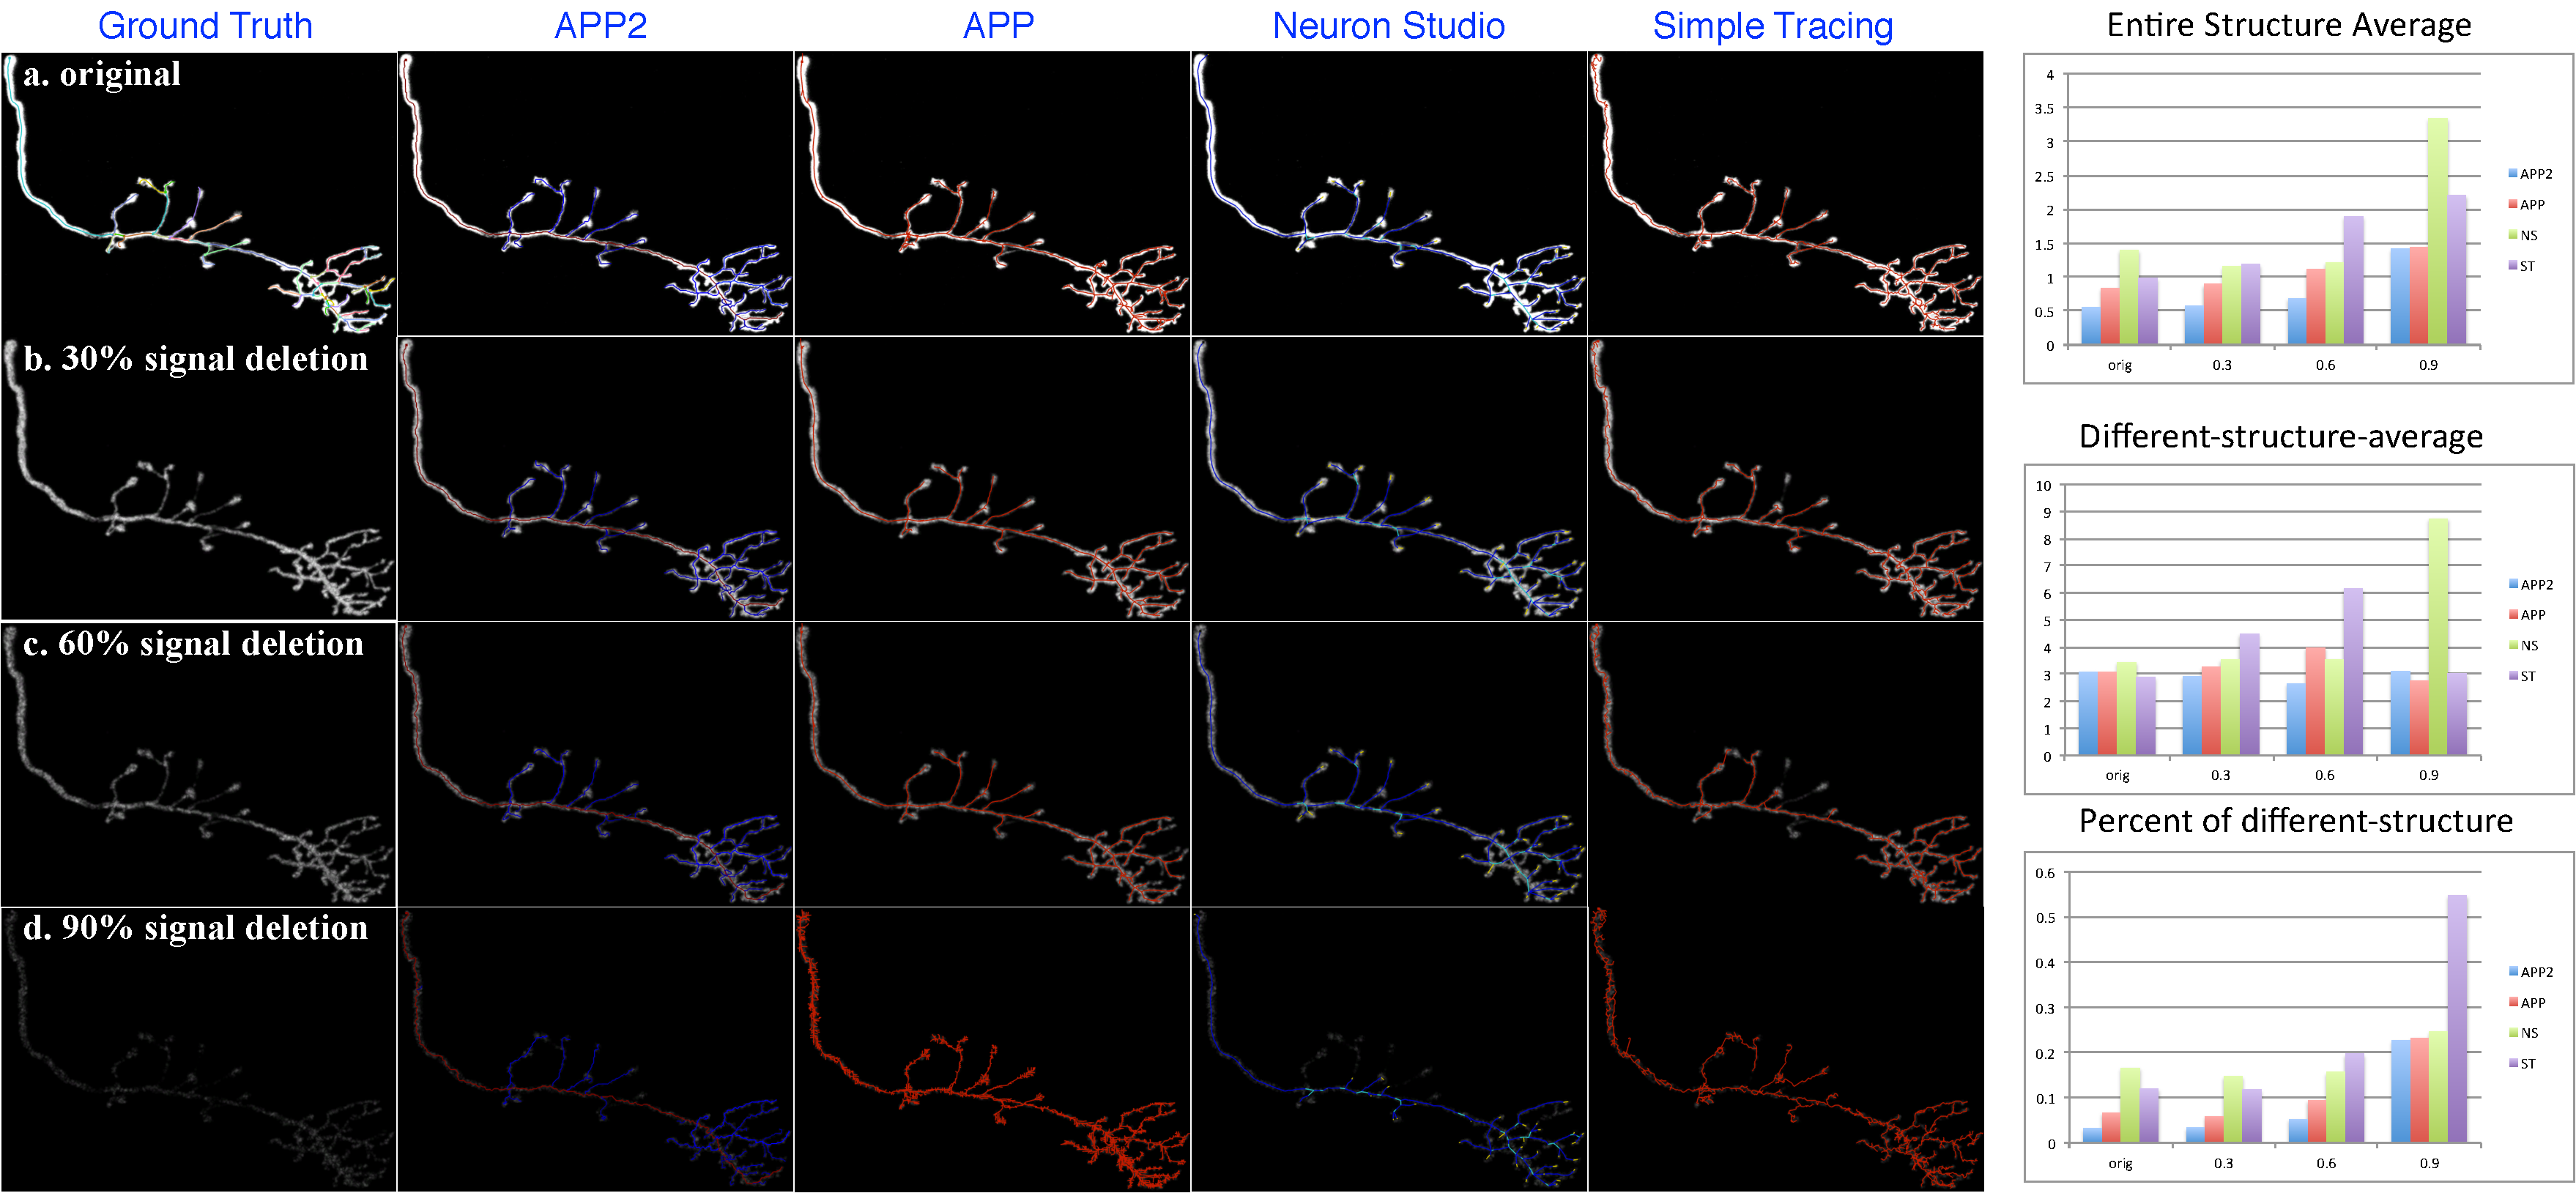
\includegraphics[width=1.0\textwidth]{images/autont_fig3}
\caption[Comparison with different neuron tracing methods subject to the deletion noise]{Comparison with different neuron tracing methods subject to the deletion noise. The reconstructions are overlaid on top of the original images for better visualization. The fourth row corresponds to 90\% signal is deleted. Since it is so dark in this case, we set pixel intensity threshold to 1 so that we are able to compare all different methods. Right side subfigures: the three difference-scores compared to the “ground truth” reconstruction. NS: NeuronStudio. ST: SimpleTracing.}
\label{fig:autont-fig3}
\end{figure}
\begin{figure}[htbp]
\centering
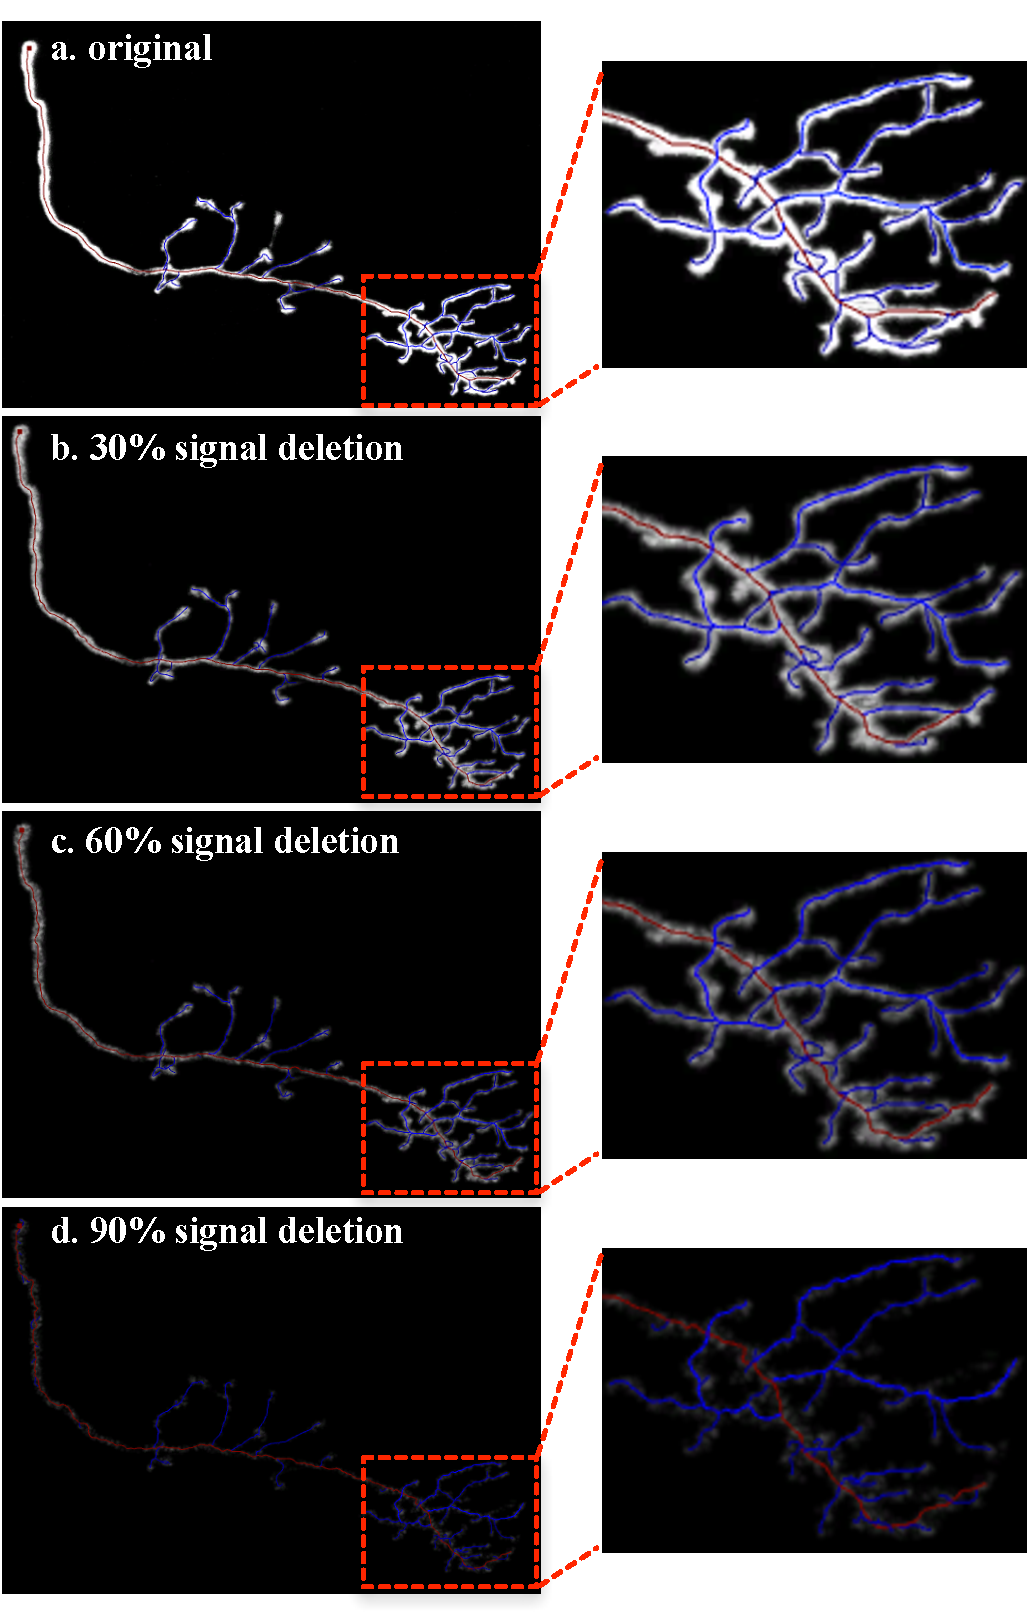
\includegraphics[width=.7\textwidth]{images/autont_fig3_2}
\caption{The signal deletion result of APP2 on Fly OP1 data}
\label{fig:autont-fig3-2}
\end{figure}

\begin{figure}[htbp]
\centering
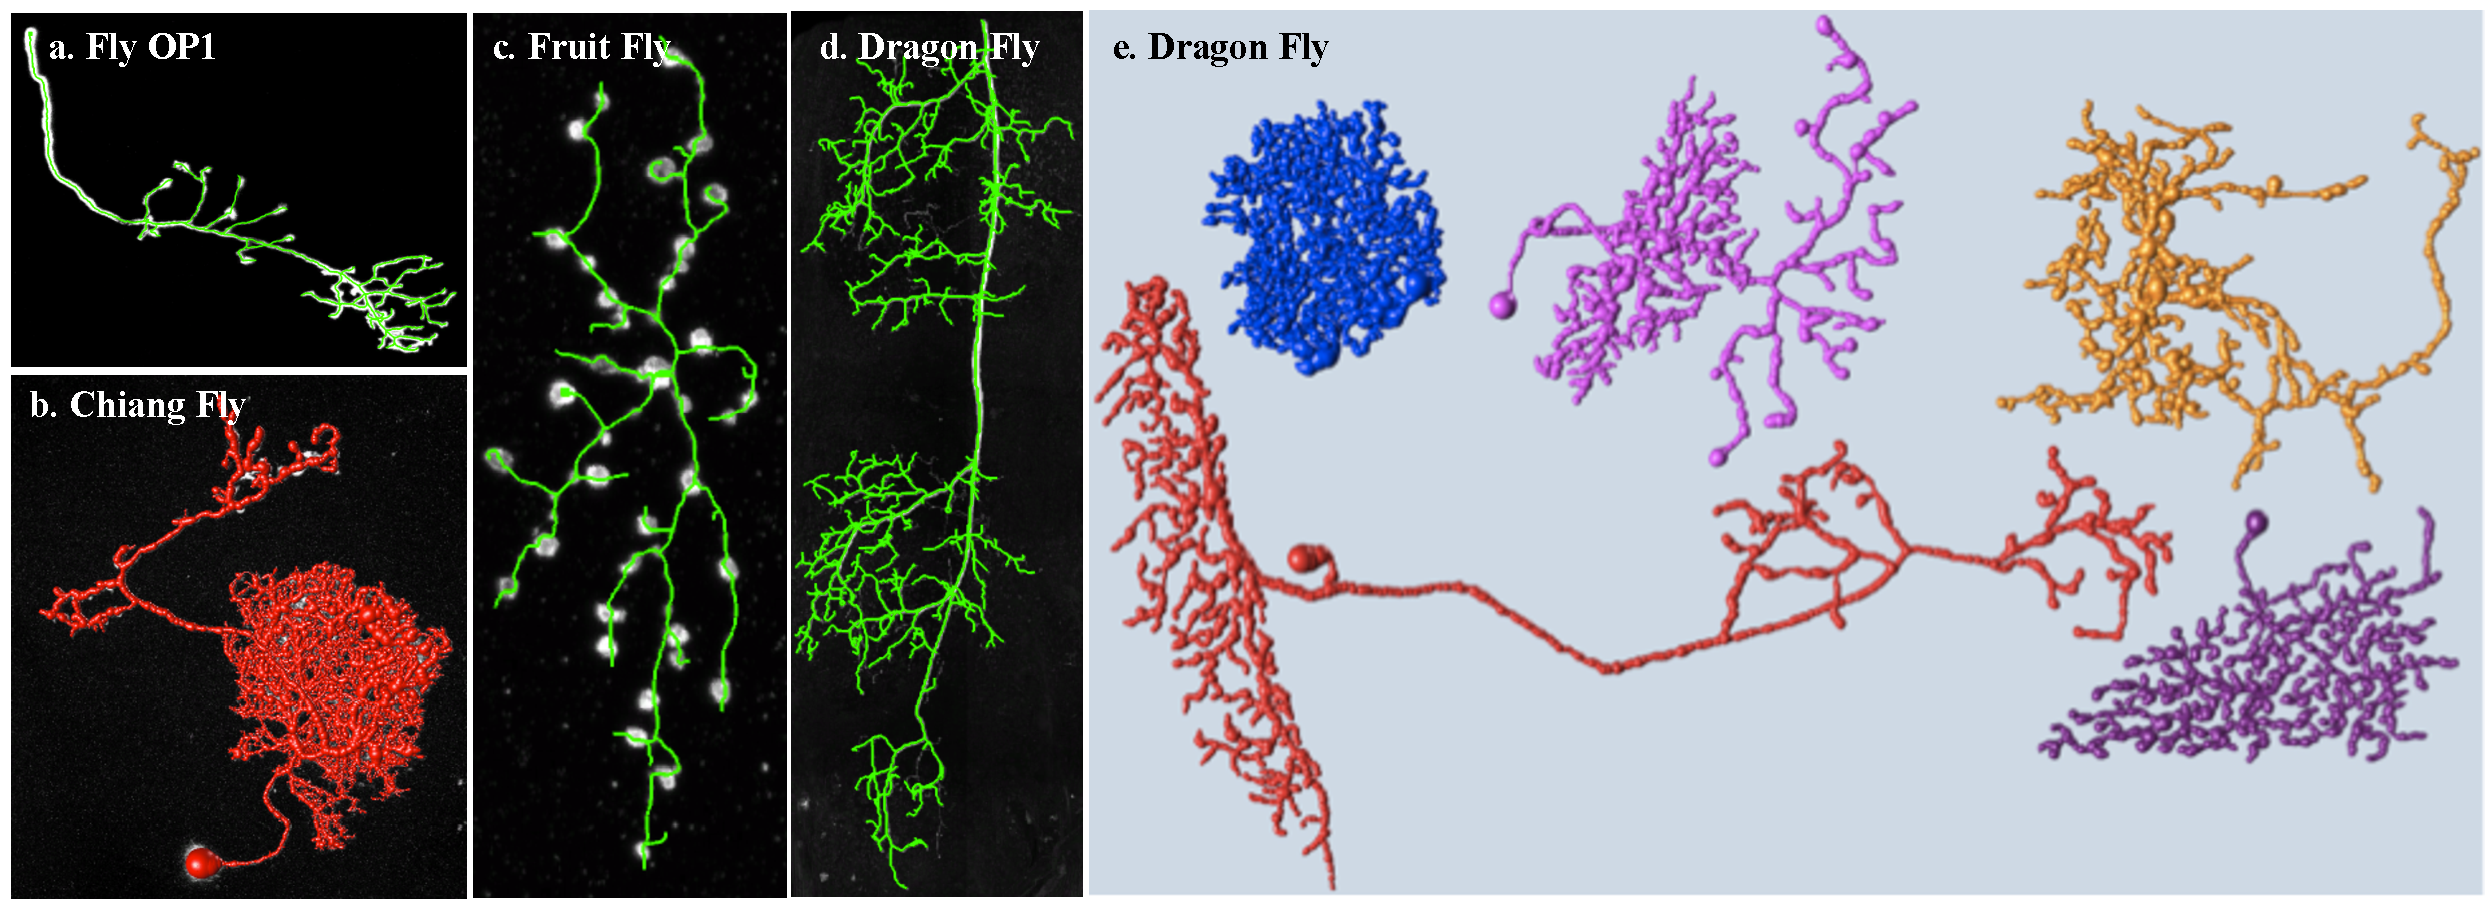
\includegraphics[width=1.0\textwidth]{images/autont_fig4}
\caption[Examples of tracing results on different neuron data sets contributed by different labs]{Examples of tracing results on different neuron data sets contributed by different labs. (a)-(d): tracing results of neurons of different model animals. (e) 3D reconstructed neurons of a large Drosophila neuron image data set with 678 neurons. Different colors indicate different neurons.}
\label{fig:autont-fig4}
\end{figure}

\section{Conclusion}
We present a new neuron tracing system that contains several novel algorithms based on fast marching and hierarchical pruning. We use the fast marching method to compute both the initial neuron reconstruction and the gray-weighted distance transform, and at the same time also improve the robustness of neuron tracing. Hierarchical pruning sorts the individual segments of an initial reconstruction tree in a hierarchical order, thus facilitates efficient removal of redundant segments in the reconstruction. We have compared our new method to various previous methods on a number of datasets and found a better performance of the new method in most cases. 
